\documentclass{article}
\usepackage[utf8]{inputenc}
\usepackage{amssymb}
\usepackage{amsmath}
\usepackage{algorithm}
\usepackage{amsthm}
\usepackage[noend]{algpseudocode}
\usepackage{filecontents}
%\usepackage{cite}
\usepackage{graphicx}
\usepackage{biblatex}
\addbibresource{interim1.bib}

\algnewcommand\INPUT{\item[\textbf{Input:}]}
\algnewcommand\OUTPUT{\item[\textbf{Output:}]}
\theoremstyle{plain} 
\newtheorem{theorem}{Theorem} 
\newtheorem{lemma}{Lemma} 

\theoremstyle{definition} 
\newtheorem{definition}{Definition} 
\newtheorem{conj}{Conjecture} 

\theoremstyle{remark} 
\newtheorem*{note}{Note} 
\newtheorem{remark}{Remark} 

\title{Most Probable String within Distance $k$\\ - interim 1 -}
\author{Yumin Kim\and Myeongjang Pyeon\and Hak-Su Lim}
\date{September 2018}


%\section{Introduction}
%hamming distance\\
%The Hamming distance between two strings of the same length is the number of different characters in the strings. That is, the minimum number of characters in the strings needed to be converted to other characters.\\\\
%most probable string\\
\begin{document}

\maketitle



\section{Probabilistic Finite-State Automata}
There are DFA/NFA that represent the accepting model to verify the acceptance of the strings, but if the probabilities is added to the transitions of the automata \cite{vidal2005probabilistic, vidal2005probabilistic2}. 
\textit{A}=$\langle\Sigma,Q,\mathbb{I_P},\mathbb{F_P},\delta_\mathbb{P}\rangle$ this is called PFA and represents the string generating model. The PFA satisfies the following conditions.\\
\begin{quotation}
\noindent
- $Q$ is a finite set of states; these will be labelled $q_1,\dots, q_{|Q|}$ unless otherwise stated\\
- $\Sigma$ is the alphabet\\
- $\mathbb{I_P}$ : Q $\rightarrow$ $\mathbb{Q^+}$ $\cap$ [0, 1] \textit{(initial-state probabilities)}\\
- $\mathbb{F_P}$ : Q $\rightarrow$ $\mathbb{Q^+}$ $\cap$ [0, 1] \textit{(final-state probabilities)}\\
- $\delta_\mathbb{P}$ : Q $\times$ ($\Sigma \cup \{\lambda\}$) $\times$ Q $\rightarrow$ $\mathbb{Q^+}$ \textit{is a transition function; the function is complete:} $\delta_\mathbb{P}$ \textit{(q,a,q') = 0 can be interpreted as "no transition from $q$ to $q'$ labelled with a". We will also denote $(q,a,q',P)$ instead of $\delta_\mathbb{P}(q,a,q') = P$ where P is a probability.}\\ 
\end{quotation}
$\mathbb{I_P}$, $\mathbb{\delta_P}$ and $\mathbb{F_P}$ are functions such that:\\
\begin{align*}
\sum_{q\in\textit{Q}}\mathbb{I_P}(q) = 1, \\
\end{align*}
\begin{align*}
and \enspace\forall q \in \textit{Q}, \mathbb{F_P}(q)+\sum_{a\in\sum\cup\{\lambda\}, q'\in\textit{Q}}\delta_\mathbb{P}(q,a,q') = 1.\\
\end{align*}
\\If the PFA generates a string, the string has a probability of being generated by the PFA. We can also find the distributions in which the strings are generated through string sampling. The distribution satisfies the following conditions.\\
\begin{quotation}
\noindent
-\textit{$Pr_D(x)$} is the probability of a string \textit{x} $\in$ $\Sigma^*$ under the distribution \textit{D} \\
-$\sum_{\textit{x}\in\Sigma^*}$ \textit{$Pr_D(x)$} = 1. \\
-$\forall q \in Q$, $\mathbb{F_P}(q)$ + $\sum_{a \in \Sigma\cup\{\lambda\}, q' \in Q}\delta_\mathbb{P}(q,a,q') = 1.$ \\
\end{quotation}
If $\lambda$-transitions are added to the PFA it is called a $\lambda$-PFA.
The PFA can be represnted with graph. Figure 1 is an example of the graph of the PFA \cite{de2010grammatical}. The numbers on the left of the state name are initial probabilities and the numbers on the right of the state name are final probabilities. The number on the 
transitions are transition probabilities. For example, the probability of parsing string "ab" with this PFA is  
\textit{$Pr_A(ab)$} that
\begin{align*}
Pr_A(ab)&= \mathbb{I_P}(q_1)\cdot\delta_\mathbb{P}(q_1,a,q_2)\cdot\delta_\mathbb{P}(q_2,b,q_4)\cdot\mathbb{F_P}(q_4)\nonumber\\
&\quad +\mathbb{I_P}(q_2)\cdot\delta_\mathbb{P}(q_2,a,q_3)\cdot\delta_\mathbb{P}(q_3,b,q_3)\cdot\mathbb{F_P}(q_3)\\
&\quad +\mathbb{I_P}(q_2)\cdot\delta_\mathbb{P}(q_2,a,q_3)\cdot\delta_\mathbb{P}(q_3,b,q_4)\cdot\mathbb{F_P}(q_4) \\
&= 0.4\cdot0.5\cdot0.4\cdot0.3\\
&\quad + 0.6\cdot0.5\cdot0.2\cdot0.4\\
&\quad + 0.6\cdot0.5\cdot0.4\cdot0.3 \\
&= 0.084
\end{align*}
\begin{figure}[htbp]
\begin{center}
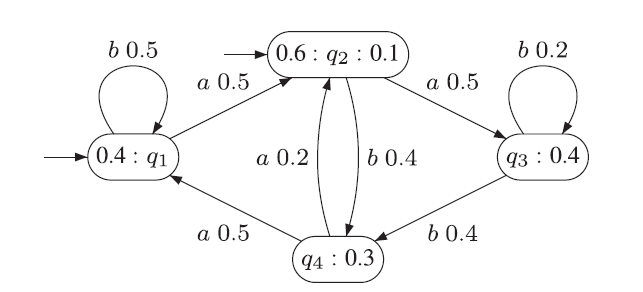
\includegraphics[scale=0.7]{figure1}
\caption{Graphical representation of a PFA \cite{de2010grammatical}} \label{fig:label}
\end{center}
\end{figure}



%%
\section{Problems}
\subsection{Related Problems}
In probabilistic automata theory, an important question is what the most probable string is. Without any constraint, the problem is called as the \textit{consensus string} problem. The formal definition is as below.\\
\textbf{Name:} Consensus string (Cs) \\
\textbf{Instance:} A probabilistic machine $\mathcal{M}$ \\
\textbf{Question:} Find in $\Sigma^{*}$ a string $x$ such that $\forall y\in \Sigma^{*}, {Pr}_{\mathcal{M}}(x) \geq {Pr}_{\mathcal{M}}(y)$.
\newline
\par
This problem can be modified as a decision problem. It is called as the \textit{most probable string} problem, defined as below. \\
\textbf{Name:} Most probable string (MPS) \\
\textbf{Instance:} A probabilistic machine $\mathcal{M}$ and $p\geq 0$ \\
\textbf{Question:} Find in $\Sigma^{*}$ a string $x$ such that ${Pr}_{\mathcal{M}}(x) > p$.
\newline
\par
If an extra constraint for the length of strings is added, it is called as the \textit{bounded most probable string} problem, which is defined as below. \\
\textbf{Name:} Bounded most probable string (BMPS)\\
\textbf{Instance:} A probabilistic machine $\mathcal{M}$, $p\geq 0$, and an integer $b$ \\
\textbf{Question:} Find in $\Sigma^{\leq b}$ a string $x$ such that ${Pr}_{\mathcal{M}}(x) > p$.
\par
\subsection{Our Problem}
In this project, we will solve another problem. In our setting, we are given a string so that the solution space is reduced to the set of string within $k-$distance with the given string. We call it as the \textit{most probable string within $k-$distance} problem and the formal definition is described as below. \\
\textbf{Name:} Most probable string within $k-$distance \\
\textbf{Instance:} A probabilistic machine $\mathcal{M}$, $p\geq 0$, a string $w$, and $k\in \mathbb{N}$ \\
\textbf{Question:} Find in $\Sigma^{*}$ a string $x$ such that ${Pr}_{\mathcal{M}}(x) > p$ and dist($x$, $w$)$\leq k$.\\
Note that the solution space is a subset of $\Sigma^{\leq |w|+k}$. So, it is not necessary to add the constraint for the length of strings.
\newline

\section{Previous Research}
% The MPS problem and the decision problem of it are NP-hard
% Suggest the bounded decision problem (BMPS) for the decision problem (NP-hard?)
% There exist a psuedo-polynomial exact algorithm to solve BMPS with PFA. (not to general probabilistic machine)

The problem of finding the most probable string (MPS) for a distribution generated by a probabilistic finite-state automaton is NP-hard.\cite{de2013most, de2013computing} Therefore the decision problem of it, which determines whether there exist a string whose probability on this machine is bigger than a given probability p, is also NP-hard. The one main reason is that there is no bound on the string. The most probable string can be of exponential length.\cite{de2013most, de2013computing}\\

We focus on the bounded decision problem of MPS(BMPS). In that case, there is an additional input integer b that bounds the length of the string lower than or equal to b. There is a pseudo-polynomial exact algorithm to solve BMPS.\cite{de2013most, de2013computing}\\

The problem we're interested in is MPS where distance within $k$ ($k$-MPS). Note that $k$-MPS is inherently a kind of BMPS because the length of string is bounded by edit(or hamming) distance $k$. There is an exact algorithm suggested by Marco Cognetta that solve this problem in pseudo-polynomial time when $k$ is lower than or equal to 1. However this algorithm cannot solve the problem in pseudo-polynomial time when $k$ is bigger than 1. We'll brainstorm how to efficiently solve $k$-MPS when $k$ is bigger than 2.


\section{Algorithms}
Firstly, we have to define some useful notations to calculate probabilities of strings generated by PFA.
\begin{definition}
Let $\mathcal{M}$ be a probabilistic automaton. Then, we define $\mathbb{I}$, $\mathbb{F}$, and $\mathbb{M}$ as matrices containing initial probabilities, final probabilities, and transition probabilities of $\mathcal{M}$.
\end{definition}
If we design a brute-force algorithm for the $k-$MPS, we have to consider all $k $ replacements of alphabets in a string and calculate its probability, which runs in $O\big(n{|\Sigma|}^{k}{n\choose k}{|Q|}^{2+O(1)} \big)$ by Le Gall algorithm \cite{le2014powers}. However, it is intractable. We can reduce some fractions of computations by using \textit{dynamic programming}. The proposed algorithm is described in Algorithm 1.
\begin{algorithm}
\caption{DP based MPS within hamming distance $k$}\label{euclid}
\begin{algorithmic}[1]
    \INPUT{a probabilistic automaton $\mathcal{M}$, a string $w$, and a distance limit $k$}
    \OUTPUT{the most probable string $w^{*}$}
    \State $n\leftarrow |w|$
    \State $\mathbb{M}_{\lambda} \leftarrow \mathrm{I}_{|Q|\times|Q|}$
    
    \State 
    $prefix(i) \leftarrow 
            \begin{cases}
                \mathbb{I}, & if \hspace{0.1cm} i=0\\
                \mathbb{I}\mathbb{M}_{w_{1}\cdots w_{i}}, & if \hspace{0.1cm} 1\leq i\leq n \\
            \end{cases}$\;
    \State 
    $suffix(i) \leftarrow 
            \begin{cases}
                \mathbb{F}, & if \hspace{0.1cm} i=n+1\\
                \mathbb{M}_{w_{i}\cdots w_{n}}\mathbb{F}, & if \hspace{0.1cm} 1\leq i\leq n \\
            \end{cases}$\;
    \State 
    $infix(i,j) \leftarrow 
            \begin{cases}
                \mathbb{M}_{w_{i}}\cdots\mathbb{M}_{w_{j}}, & if \hspace{0.1cm} 1\leq i\leq j\leq n\\
                \mathrm{I}_{|Q|\times|Q|}, & if \hspace{0.1cm} i>j \\
            \end{cases}$\;
            
    \State $w^{*} \leftarrow \lambda$
    \State $p^{*} \leftarrow 0$

    \For{each $k$-combination $\sigma$ of $n$}
        \For{each $(c_{1},\cdots, c_{k})\in \Sigma^{k}$}
            \State $w'\leftarrow$ a string obtained by replacing $w_{\sigma(i)}$ by $c_{i}$ for all $1\leq i \leq k$
            \State $p(w')\leftarrow prefix(\sigma(1)-1)$
            \For{$i\leftarrow 1,\cdots, k-1$}
                \State $p(w')\leftarrow p(w')\mathbb{M}_{c_{i}}infix(\sigma(i)+1,\sigma(i+1)-1)$
            \EndFor
            
            \State $p(w')\leftarrow p(w')\mathbb{M}_{c_{k}}suffix(\sigma(n)+1)$
            \If{$p^{*}<p(w^{\prime})$}
                \State $w^{*} \leftarrow w^{\prime}$
                \State $p^{*} \leftarrow p(w')$
            \EndIf
        \EndFor
    \EndFor
    \State \Return $w^{*}$
\end{algorithmic}
\end{algorithm}
\begin{theorem}
The string obtained by Algorithm 1 is the most probable string within distance $k$.
\end{theorem}
\begin{proof}
It is trivial that the calculation of probabilities is correct. So, now we assume it and prove that the obtained string is the most probable string. Suppose that there exists $w^{\prime}$ such that $d_{hamming}(w,w^{\prime})=k^{'}\leq k$ and $p(w^{\prime})>p(w^{*})$. Then, $p(w^{\prime})>p(w_{0})$ for all strings obtained by replacing $k$ or less characters in $w$ with others. Since $d_{hamming}(w,w^{\prime})\leq k$, it is considered at line 10. Thus, $w^{\prime}=w^{*}$, which contradicts to the assumption.
\end{proof}
\begin{theorem}
Algorithm 1 runs in $O\big( n^{2}{|Q|}^{2+O(1)}+k{|\Sigma|}^{k}{n\choose k}{|Q|}^{2+O(1)}\big)$.
\end{theorem}
\begin{proof}
Note that the running time of matrix multiplication of $A_{n\times m}$ and $B_{m\times p}$ is $O(nmp)$. However, if $n=m=p$, we can calculate it in $O\big(n^{2+O(1)}\big)$ by Le Gall algorithm \cite{le2014powers}. So, we can calculate $prefix$, $suffix$, and $infix$ in $O\big(n^{2}{|Q|}^{2+O(1)} \big)$ and $w^{*}$ in $O\big(k{|\Sigma|}^{k}{n\choose k}{|Q|}^{2+O(1)} \big)$. Thus, the total running time is $O\big( n^{2}{|Q|}^{2+O(1)}+k{|\Sigma|}^{k}{n\choose k}{|Q|}^{2+O(1)}\big)$.
\end{proof}
\iffalse
\begin{algorithm}
\caption{intersection based MPS within hamming distance $k$}\label{euclid}
\begin{algorithmic}[1]
    \INPUT{a probabilistic automaton $\mathcal{M}$, a string $w$, and a distance limit $k$}
    \OUTPUT{the most probable string $w^{*}$}
    \Procedure{Normalize}{$\mathcal{M}$}
    % To do: Yu-Min
    \For{each $q_i \in Q$}
    \EndFor
    \EndProcedure
    \State $\mathcal{A}\leftarrow $ construct a Levenshtein automaton with $w$ and $k$
    \State $\mathcal{M}^{\prime}\leftarrow \mathcal{M}\cap \mathcal{A}$
    \State $\mathcal{M\prime}\leftarrow $remove all lambda transitions in $\mathcal{M}^{\prime}$
    \State $\mathcal{M}^{\prime}\leftarrow $\textsc{Normalize}$(\mathcal{M}^{\prime})$
    \State $w^{*} \leftarrow$ \textsc{MPS}$(\mathcal{M}^{\prime})$
    \State \Return $w^{*}$
\end{algorithmic}
\end{algorithm}
\fi
\section{Implementation}
We implemented a PFA framework based on Python. In order to boost the performance, we used the Numpy library for parallel matrix processing. The detailed class structures are depicted in Figure 2.
% Todo: Yumin implementation_diagram.png
\begin{figure}[htbp]
\begin{center}
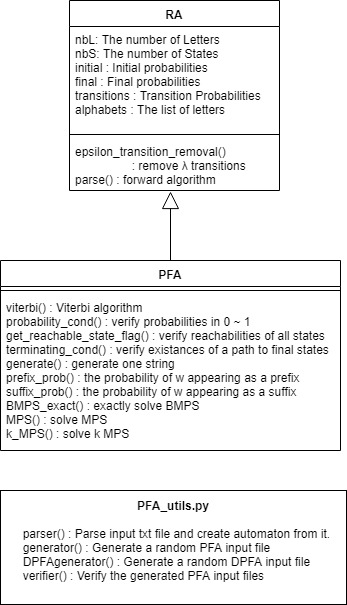
\includegraphics[scale=0.4]{implementation_diagram}
\caption{Class and function diagram of our implementation} \label{fig:label}
\end{center}
\end{figure}
\section{Experiments}
In order to compare our algorithm to the brute-force algorithm, we implemented both algorithms and test as adjusting $n$ and $k$ by sampling DPFA and strings. We sampled $10$ DPFA and $100$ strings per each $n$ and $k$ pair. 

\begin{figure}[htbp]
\begin{center}
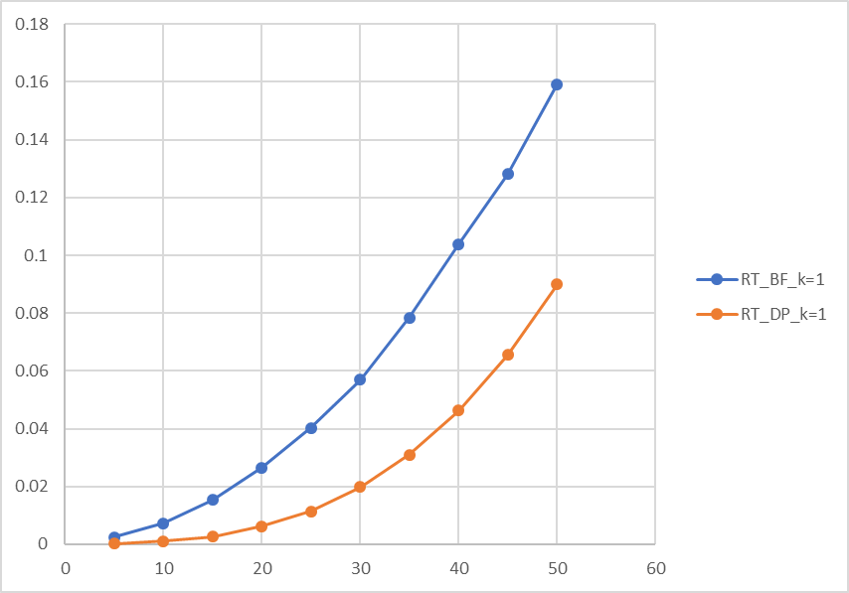
\includegraphics[scale=0.7]{RT_BF_DP_k-1}
\caption{Running time chart when k = 1} \label{fig:label}
\end{center}
\end{figure}

\begin{figure}[htbp]
\begin{center}
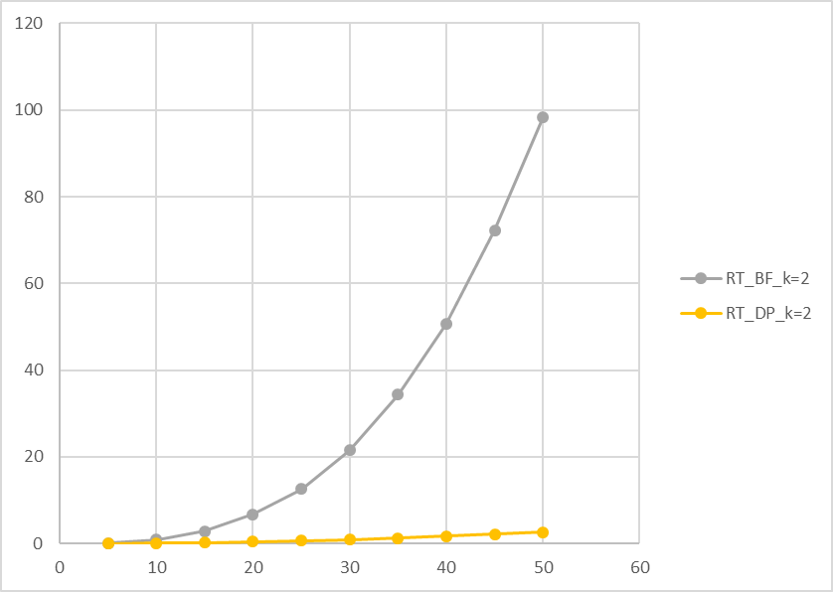
\includegraphics[scale=0.7]{RT_BF_DP_k-2}
\caption{Running time chart when k = 2} \label{fig:label}
\end{center}
\end{figure}

\begin{figure}[htbp]
\begin{center}
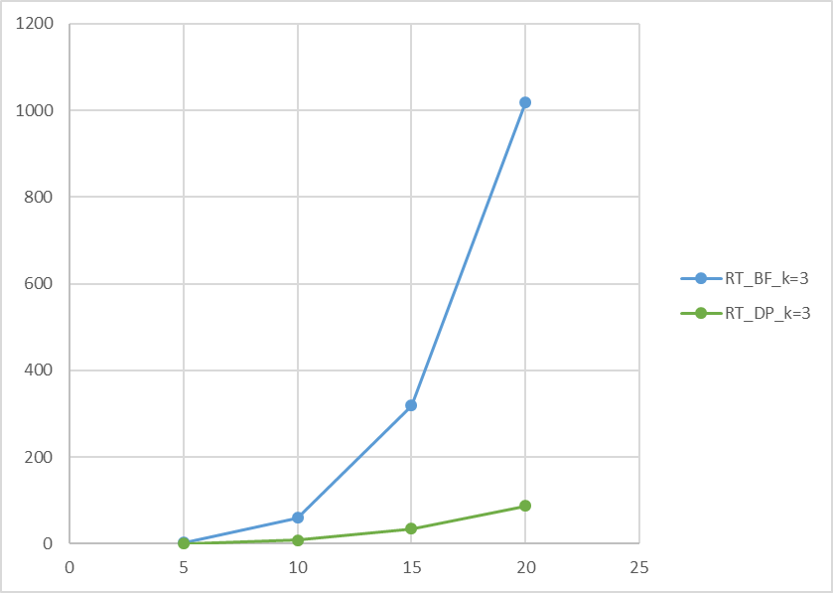
\includegraphics[scale=0.7]{RT_BF_DP_k-3}
\caption{Running time chart when k = 3} \label{fig:label}
\end{center}
\end{figure}

\clearpage
\printbibliography

\end{document}
